\chapter{Revisão da Literatura}

Para propor uma metodologia que permita validar o ETHEL se faz necessário uma revisão na literatura para construção do embasamento teórico, essencial para a construção desse trabalho. Este capítulo apresenta a revisão literária realizada.
%Neste capítulo será demonstrado a teoria do estudo em questão, apresentando outras literaturas que foram utilizadas para construção do embasamento teórico necessário para a construção desse trabalho.

\section{Posturografia}

O comprometimento do equilíbrio é comum em pessoas idosas e em pacientes com diversos tipos de doenças, incluindo patologia vestibular, disfunções visual ou oculomotor, doenças neurológicas e distúrbios musculoesqueléticos (\citeauthor{visser2008clinical}, \citeyear{visser2008clinical}). Os pacientes portadores de distúrbios de equilíbrio sofrem com a possibilidade eminente de queda que pode levar a fraturas, gerando insegurança e impactando negativamente a qualidade de vida. Neste contexto, se faz necessário ter acompanhamento médico, tanto para diagnóstico quanto para tratamento das patologias causadores do desequilíbrio.

Identificar de maneira correta os pacientes que tem risco de quedas, é um desafio clínico. Vários testes clínicos, são capazes de identificar pessoas com risco de quedas razoavelmente bem, como por exemplo,  \textit{Berg Balance Scale} (\citeauthor{berg1992measuring}, \citeyear{berg1992measuring}), o \textit{Functional Reach Test} (\citeauthor{duncan1990functional}, \citeyear{duncan1990functional}), o teste de 10 metros  (\citeauthor{rossier2001validity}, \citeyear{rossier2001validity}) o teste \textit{“Up-and-go”}  (\citeauthor{podsiadlo1991timed}, \citeyear{podsiadlo1991timed}). Mas o número de predições falso-negativa ainda é alto em alguns destes testes (\citeauthor{bloem2006posture}, \citeyear{bloem2006posture}). Além do mais, a execução dos mesmos muda consideravelmente entre diferentes médicos e a interpretação dos resultados e variável devido ao sistema de pontuação subjetivo.

 O controle da postura é mantido por um sistema sensorimotor complexo, que integra informações dos sistemas visual, vestibular e somatossensorial. A integridade do sistema de controle postural é habitualmente avaliado com testes de posturografia estática e/ou dinâmica e, é em geral mensurada com base no deslocamento do centro de pressão (COP) medido com uma uma plataforma de força, que também mede as forças de reação vertical e horizontal. O COP é a localização da reação vertical na superfície de uma plataforma de força, ele reflete as orientações dos ângulos articulares do corpo, bem como os seus movimentos para manter o centro de gravidade sobre sua base suporte (\citeauthor{lafond2004intrasession}, \citeyear{lafond2004intrasession}).

Tendo isso em vista, a posturografia é utilizada como uma importante técnica para avaliar as alterações posturais e as oscilações corporais. Técnicas posturograficas são utilizadas para averiguar a regulação ativa e passiva do equilíbrio sob diversas condições. O equilíbrio é geralmente testado quantitativamente em experimentos de laboratório (\citeauthor{browne2000development}, \citeyear{browne2000development}). O dispositivo comumente utilizado para isso é uma plataforma de força.  A PF possui sensores de força acoplados a uma placa que são responsáveis por determinar a localização centro de pressão (COP) (\citeauthor{leach2014validating}, \citeyear{leach2014validating}). A  maioria das técnicas de posturografia são realizadas manipulando a postura ou o equilíbrio, afim de avaliar a resposta do paciente a tais procedimentos. A posturografia computadorizada fornece medidas objetivas e quantitativas do equilíbrio e, das oscilações corporais. Ao contrário dos testes clínicos, o avaliador pode especificar os parâmetros de avaliação, podendo introduzir várias manipulações para tornar o controle postural mais desafiador. Também é possível usar perturbações sensoriais para manipular seletivamente um ou mais elementos específicos do controle postural. Desta forma, pode ser fornecido ao examinador resultados melhores e mais específicos, contribuindo para identificação  das possíveis causas do desequilíbrio (\citeauthor{visser2008clinical}, \citeyear{visser2008clinical}).


Na posturografia estática, o paciente é avaliado de acordo com o desempenho do seu sistema de controle postural, de pé e quieto sobre uma superfície fixa. Geralmente as avaliações incluem, teste com olhos abertos e com olhos fechados. Assim é possível estimar o papel do sistema visual na manutenção equilíbrio permanente. Na posturografia dinâmica, o desempenho do sistema de controle dinâmico é medido através da resposta, dada uma pertubação aplicada ou volitiva. Com isso, é possível estimar algumas métricas como a reação postural defensiva imediata, tempo de reação, excursão máxima e o controle direcional (\citeauthor{prieto1996measures}, \citeyear{prieto1996measures}).


\section{Plataformas de Força}
As plataformas de força foram criadas, com intuito de avaliar uma variedade de áreas, incluindo a reabilitação neurológica, desempenho atlético e prevenção de quedas em idosos, plataformas de força pode fornecer informações quantitativas detalhadas sobre déficits de movimento ou mecanismos de controle postural, e respostas a manipulações sensoriais. Normalmente medem
forças e momentos de reação, que são utilizados no calculo do desenvolvimento da
posição e na posição do centro de pressão (COP)  (\citeauthor{clark2018reliability}, \citeyear{clark2018reliability}).

De modo geral, uma plataforma de força consiste em uma placa sobre alguns sensores de força (geralmente quatro) do tipo célula de carga ou piezoelétrico, que estão distribuídos, afim de medir três componentes da força empregada neles, Fx, Fy e Fz (x, y e z são as direções ântero-posterior, médio-lateral e vertical, respectivamente), e os três componentes do momento de força (ou torque), Mx, My e Mz, agindo sobre a plataforma (\textbf{Figura \ref{PF}}) (\citeauthor{duarte2010revision}, \citeyear{duarte2010revision}).

\begin{figure}
\captionsetup{justification   = raggedright,
              singlelinecheck = false}
\caption{Representação das forças obtidas por meio dos sensores
da plataforma de força}\label{PF}
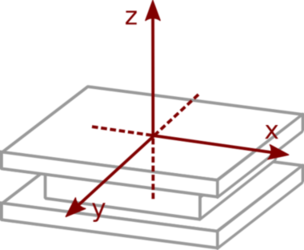
\includegraphics[width=0.7\textwidth]{figs/PF1.png}
\end{figure}

Medidas do equilíbrio estático derivados da plataforma de força tem contribuído na avaliação da importância de diferentes sistemas sensoriais no controle do equilíbrio (\citeauthor{shumway1986assessing}, \citeyear{shumway1986assessing}), na predição de ocorrências de quedas (\citeauthor{pajala2008force}, \citeyear{pajala2008force}) e para avaliar a eficácia de protocolos de treinamento utilizados na manutenção do equilíbrio (\citeauthor{bonan2004reliance}, \citeyear{bonan2004reliance}). No entanto, o acesso a essa tecnologia é limitada devido ao alto custo das plataformas de força e especialização necessária para utilizá-las (\citeauthor{visser2008clinical}, \citeyear{visser2008clinical}).


\section{O uso da WBB na realização de exames posturográficos}\label{UsoDaWBB}

A Plataforma WBB, foi lançada em 2007 como um controle de jogo para o sistema Nitendo \textit{Wii}, desenvolvida com o objetivo de promover uma maior imersão do usuário ao jogo. A WBB possui componentes similares a uma plataforma de força tradicional, dispõe de quatro sensores de carga medidores de tensão (\textbf{Figura \ref{sensoresWBB}}), capazes de obter dados sobre movimentos no COP e comunicar-se via bluetooth com um computador. Ela foi avaliada como uma alternativa as plataformas de força de nível laboratorial, devido ao seu baixo custo relativo e por ser de fácil manuseio (<4 kg) (\citeauthor{clark2018reliability}, \citeyear{clark2018reliability}).


\begin{figure}
\captionsetup{justification   = raggedright,
              singlelinecheck = false}
\caption{Identificação dos sensores de força na WBB}\label{sensoresWBB}
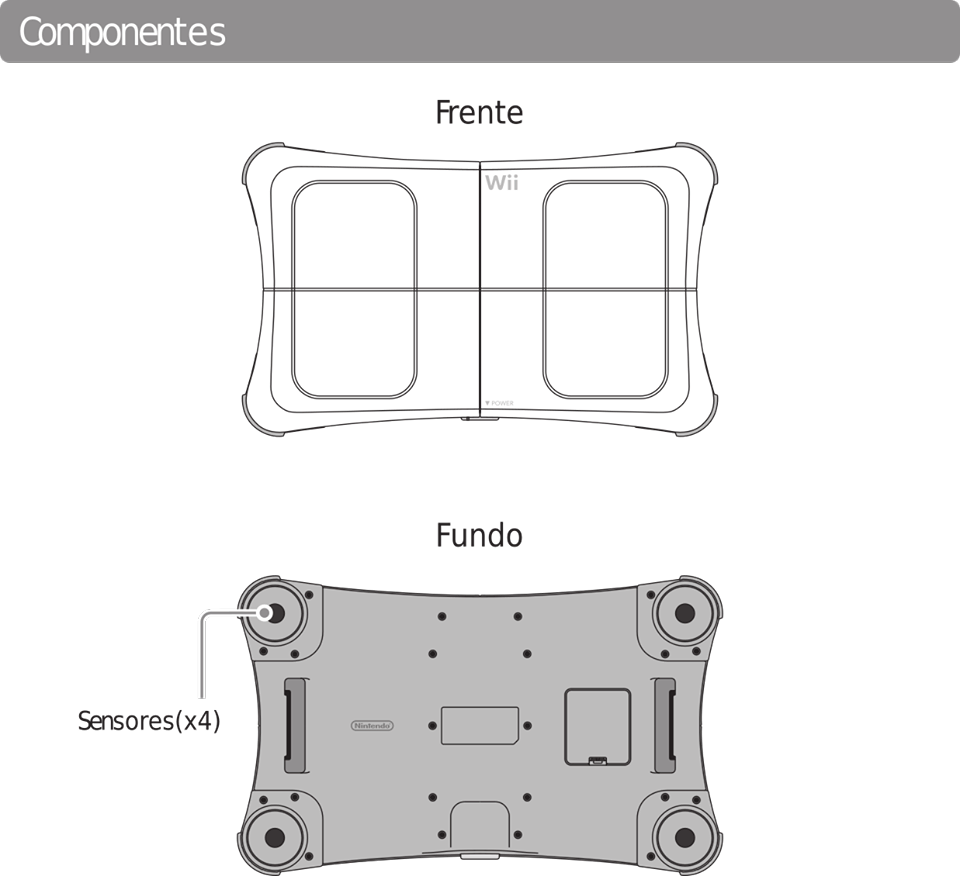
\includegraphics[width=1.0\textwidth]{WBB.png}
\footnotesize Fonte: Nintendo, Operations Manual, p.3
\\\footnotesize Nota: Adaptado e traduzido pelo o autor
\end{figure}

A maioria dos estudos que averígua o uso do WBB atestaram sua confiabilidade e validade quando comparado com plataformas de força tradicionais, aplicadas na avaliação do equilíbrio de pé (\citeauthor{clark2010validity}, \citeyear{clark2010validity}),  (\citeauthor{young2011assessing}, \citeyear{young2011assessing}), (\citeauthor{huurnink2013comparison}, \citeyear{huurnink2013comparison}), (\citeauthor{leach2014validating}, \citeyear{leach2014validating}). A WBB também já foi aplicada como ferramenta de medição, utilizando um grande número de pacientes clínicos (\citeauthor{clark2017standing}, \citeyear{clark2017standing}), (\citeauthor{clark2017standing414}, \citeyear{clark2017standing414}).


Clark et al. (\citeyear{clark2010validity}) efetuou um trabalho que visava analisar a validade e confiabilidade do WBB na avaliação do equilíbrio permanente. Para isso, foi feita a comparação dos dados do COP coletados em uma WBB com o de uma PF laboratorial durante uma variedade de testes de equilíbrio. Trinta indivíduos saudáveis, que não apresentava histórico de doenças neurológicas e patologias importantes nas costas ou membros inferiores que pudesse influenciar o equilíbrio participaram dos testes. Os participantes realizaram uma série de quatro tarefas de equilíbrio permanente em uma PF de nível laboratorial (Modelo AMTI OR6-5,Watertown, MA, E.U.A.), calibrado de acordo com as recomendações do fabricante. Para utilizar a WBB foi usado o software customizado (\textit{Labview 8.5 National Instruments}, Austin, TX, E.U.A.), ela foi calibrada colocando uma variedade de cargas conhecidas em diferentes posições na WBB. Ao fim dos experimentos, os autores concluíram que a WBB fornece dados comparáveis a uma PF comercial na avaliação do COP, e que a WBB é um dispositivo satisfatório para avaliar o equilíbrio. Além disso, pode fornecer aos profissionais da saúde informações importantes e suplementares sobre o equilíbrio que não são perceptíveis usando apenas a avaliação visual. Sendo assim, a WBB poderia ser uma alternativa de baixo custo na avaliação clínica do equilíbrio, substituindo os tradicionais protocolos de avaliação subjetiva e visual. As principais limitações ficaram por conta da incapacidade de avaliação da força no eixo horizontal e pela necessidade de personalização de um \textit{software} para fazer a interface da WBB com o computador.

\cite{young2011assessing} propôs uma nova abordagem na utilização da WBB para avaliação e treinamento do equilíbrio permanente em idosos, para isso, foram   projetados dois jogos. O primeiro demandava do participante o controle da posição médio-lateral do seu COP em uma tentativa de pegar maçãs caindo de uma árvore. O segundo jogo exigia tanto controle médio-lateral quanto anterior-posterior do COP para manipular a posição de um personagem na tentativa de se mover em uma direção para estourar bolhas. Para avaliar a efetividade da interface criada, foram recrutados seis voluntários (1 homem, 5 mulheres), que participaram de 10 sessões utilizando os jogos (20 min cada) durante um período de quatro semanas.
Após o treinamento, quando perguntado se os participantes optariam por continuar jogando os jogos de equilíbrio durante um período mais longo (por exemplo, seis meses), todos responderam “definitivamente sim”. Além disso, todos os participantes relataram ter gostado da experiência de jogo e apresentam uma melhora média de 11\%  na escala \textit{Tinetti's Falls Efficacy Scale} (\citeauthor{tinetti1990falls}, \citeyear{tinetti1990falls}) pós-treinamento em comparação ao pré-treinamento, refletindo uma maior confiança na capacidade de realizar tarefas funcionais.

Huurnink et al. (\citeyear{huurnink2013comparison}) realizou um estudo comparativo entre as plataformas de forças de laboratório com a WBB, na medição do controle postural em tarefas de equilíbrio. Apos a realização de testes com quatorze voluntários, Huurnink et al. (\citeyear{huurnink2013comparison}) concluiu que apesar das limitações como a baixa taxa de amostragem e significativa taxa de ruídos, a WBB é suficientemente precisa para quantificar a trajetória do COP, amplitude e velocidade total durante as
tarefas de equilíbrio, e que a WBB apresenta uma boa correspondência com os resultados obtidos através da PF. Além disso, a estimativa da localização instantânea do COP é bastante semelhante a localização obtida com a PF. Das tarefas avaliadas, houve uma boa correspondência nas medidas das trajetórias do COP, o que sugere que qualquer medida de equilíbrio baseada na trajetória do COP feita com a WBB, pode ser considerada suficientemente precisa. Huurnink et al. (\citeyear{huurnink2013comparison}) afirma que várias áreas (por exemplo, esportes, medicina esportiva e medicina de reabilitação) podem se beneficiar da implementação em larga escala da WBB, devido a seu baixo custo.

Apesar de todos os aspectos positivos, os autores  Pagnacco, Oggero e Wright (\citeyear{pagnacco2011biomedical}) falam que a WBB é limitada. Das limitações elencadas podem se destacar, a baixa e inconsistente taxa de amostragem, o fato de ter uma quantidade significativa de ruído nos dados, a característica de que sua amostragem não é sincronizada entre os quatro sensores de força e possuir limitações mecânicas e eletrônicas. Segundo os autores a quantidade significativa de ruídos nos dados adquiridos com uma WBB pode ser atribuído aos cabos não blindados e sua eletrônica incapaz de reduzir o ruído. Pagnacco, Oggero e Wright (\citeyear{pagnacco2011biomedical}) mediram simultaneamente o deslocamento do COP com a WBB e a PF e, ao contrário dos trabalhos citados anteriormente, os autores optaram por não utilizar uma calibração personalizada na WBB. Em vez disso, usaram o vetor de calibração padrão, armazenado internamente pelo fabricante. Eles argumentaram que um método de calibração personalizado é caro, consome muito tempo e não é acessível nem viável para a maioria dos usuários. Além disso, segundo Pagnacco, Oggero e Wright (\citeyear{pagnacco2011biomedical}), a calibração personalizada proposta por Clark et al. (\citeyear{clark2010validity}), tem efeito mínimo sobre o ruído inerente aos dados da WBB. Dadas as limitações, Pagnacco, Oggero e Wright (\citeyear{pagnacco2011biomedical}) não recomendam a utilização da WBB para outros fins que não seja para o que foi criada, isto é, como um brinquedo.

\cite{leach2014validating} realizou um estudo com o objetivo de validar a WBB comparado com uma PF "padrão ouro", quantificando o erro de medição do COP utilizando a WBB. Um segundo objetivo foi determinar a variabilidade entre dispositivos WBB (para isso utilizaram 12 WBBs diferentes). Além das WBBs, foi usada uma plataforma de força (AMTI OR6-6, Watertown, MA, EUA) para medir simultaneamente com a WBB o deslocamento unidimensional do COP de sinais dinâmicos de entrada/saída controlados. No experimento de validação a WBB foi colocada sobreposta à plataforma de força e acima delas foi colocado um sistema mecânico de pêndulo invertido que era responsável por simular oscilações posturais unidimensionais. Dadas as oscilações, realizava-se a aquisição dos dados gerados por ambas plataformas. As principal limitação listada pelos autores foi a composição material da plataforma, por ser de plástico ela é suscetível à deformação elástica quando uma carga significativa é aplicada. Se a superfície se deforma durante a aquisição de dados, a capacidade da WBB de adquirir medições precisas de CoP pode ser prejudicada. Além disso, a WBB é incapaz de medir momentos e forças horizontais. Ao fim do estudo, os autores concluíram que a utilização de um protocolo de calibração, reduziu significativamente os erros e minimizou a variabilidade entre dispositivos, o que, por sua vez, fortaleceu a confiabilidade e indicou baixa variabilidade entre dispositivos WBBs. No entanto, os autores não recomendam o uso da WBB como ferramenta de diagnóstico clínico, acreditam que a WBB poderia substituir a PF somente em situações em que precisão e exatidão mais baixas são acetáveis, como monitoramento de oscilação postural em idosos, em pequenas clínicas ou ambiente doméstico. Ademais, confirmam que o dispositivo e o \textit{software} usados para adquirir dados com a WBB, podem afetar a qualidade das medidas do COP derivadas dos dados da WBB.


Tento em vista essas divergências entre autores, foi realizada uma revisão sistemática por \cite{clark2018reliability} com o propósito de avaliar a confiabilidade e a validade da WBB para avaliação do equilíbrio. Os resultados da revisão sistemática indicaram que a WBB pode fornecer dados que são válidos quando comparados com os dados das plataformas de força comercial, possuindo características de confiabilidade para realização da posturografia computadorizada. Dos trabalhos levantados, 21 examinaram a validade concorrente da WBB (ou seja, a comparação com outra plataforma de força) e, em geral, a WBB demostrou ser excelente quando examinada a associação dos dados capturados em ambos dispositivos. Entretanto, a WBB possui limitações (por exemplo, inconsistência na taxa de amostragem e ruídos no sinal), mas essas limitações podem ser amenizadas, com um boa implementação do protocolo de aquisição de dados, com métodos de filtragem de sinais e seleção de variáveis. Com isso, o erro inerente a este dispositivo é minimizado e sua confiabilidade e validade é maior.

\section{Softwares de aquisições de dados utilizando  a WBB}

Na seção \ref{UsoDaWBB} vimos que muitos são os estudos que visam avaliar e validar a utilização da WBB na realização de exames posturográficos, em testes e tratamentos do equilíbrio. Contudo, poucos são os estudos que analisam o desenvolvimento de \textit{softwares} para fazer a interface da WBB com o computador. Além da aquisição e quantificação dos dados gerados, afim de obter resultados objetivos e confiáveis. Apesar da escassez de estudos nesse âmbito, alguns autores destacam a importância dos softwares de coleta de dados com a WBB, por exemplo, Huurnink et al.,(\citeyear{huurnink2013comparison}) confirmam que o dispositivo e o software utilizados para fazer a interface e a captura dos dados com a WBB, podem afetar a qualidade das medidas do COP derivadas dos dados da WBB. Na revisão sistemática feita por Clark et al. (\citeyear{clark2018reliability}), percebe-se que a maioria dos autores constrói rotinas em softwares de terceiros (principalmente o \textit{LabVIEW}) para aquisição e leitura de dados. A principal limitação do uso dessa solução, é que geralmente estes softwares utilizados são softwares proprietários e suas licenças são dispendiosas. Além disso, geralmente é necessário realizar a personalização desses softwares, para adaptação dos mesmos visando o uso com a WBB (\citeauthor{clark2010validity}, \citeyear{clark2010validity}).

%(\citeyear{clark2010validity}) customizou o software Labview para fazer a interface entre WBB e o computador, e para  aquisição de dados. Mas os autores destacam que a necessidade de personalização de um software para fazer a interface da WBB com o computador pode se tornar uma limitação para uso da mesma, tendo em vista, que a maioria dos profissionais da área da saúde (público alvo) não possuem habilidades técnicas necessárias para criação e/ou personalização de programas. Além disso, os autores propõem como pesquisa adicional, a criação de um software para facilitar a avaliação do equilíbrio com a WBB no ambiente clínico.



Segundo Park e Lee (\citeyear{park2014validity}) há poucos \textit{softwares} projetados para testar o equilíbrio utilizando a WBB e poucos são os estudos sobre a confiabilidade e validade dos mesmos. Sendo assim, foi desenvolvido e validado por eles o \textit{software balancia} (\textit{Balancia} v1.0, sistemas Minto, Seul, República da Coreia). O \textit{software Balancia} foi desenvolvido utilizando C++ e \textit{LabVIEW}. A confiabilidade e validade foram confirmadas comparando os resultados obtidos com o \textit{balancia} utilizando a WBB com um PF de nível laboratorial. Vinte adultos saudáveis participaram dos testes. Dados como o COP e a velocidade do COP foram adquiridos dos sistemas de avaliação. A confiabilidade da validade concorrente foi analisada por um coeficiente de correlação intraclasse (ICC). Como resultado obtiveram validade concorrente (ICC: 0,87-0,73). Sendo assim, concluíram que o \textit{software Balancia} pode ser considerado um dispositivo de avaliação confiável e em conjunto com a WBB podem ser utilizados em ambientes clínicos para a avaliação do equilíbrio. No entanto, o \textit{software} \textit{Balancia} não se encontra disponível de forma gratuita e também, após pesquisa, o \textit{software} não foi encontrado para aquisição.

Llorens et al. (\citeyear{llorens2015low}), projetaram uma ferramenta  baseada na web (\textit{Posturography Test,  Neurorehabilitation & BrainResearch Group}) que permite aos médicos realizar avaliações posturográficas utilizando a WBB. A ferramenta está disponível gratuitamente para o público. É necessário instalar um programa localmente para executar os exercícios, recuperar os dados da WBB e carregar os resultados na página Web do sistema. Depois disso os resultados são comparados com o desempenho de uma amostra correspondente que está salvo em uma base de dados. Por fim, os resultados são apresentados ao usuário (\textbf{Figura \ref{pTeste}}). Segundo os autores a plataforma WEB foi programada em ASP.NET usando o Visual Studio (Microsoft®, WA). O SQL Server (Microsoft®, WA) foi usado para desenvolver o banco de dados. O ambiente virtual que retrata os exercícios foi projetado usando o 3D GameStudio (\textit{Conitec Datensysteme GmbH}, Alemanha). E a WBB é conectada ao computador via tecnologia \textit{Bluetooth}.

\begin{figure}
\captionsetup{justification   = raggedright,
              singlelinecheck = false}
\caption{Exemplo de parte dos resultados apresentado pelo \textit{Posturography Test} aos usuários}\label{pTeste}
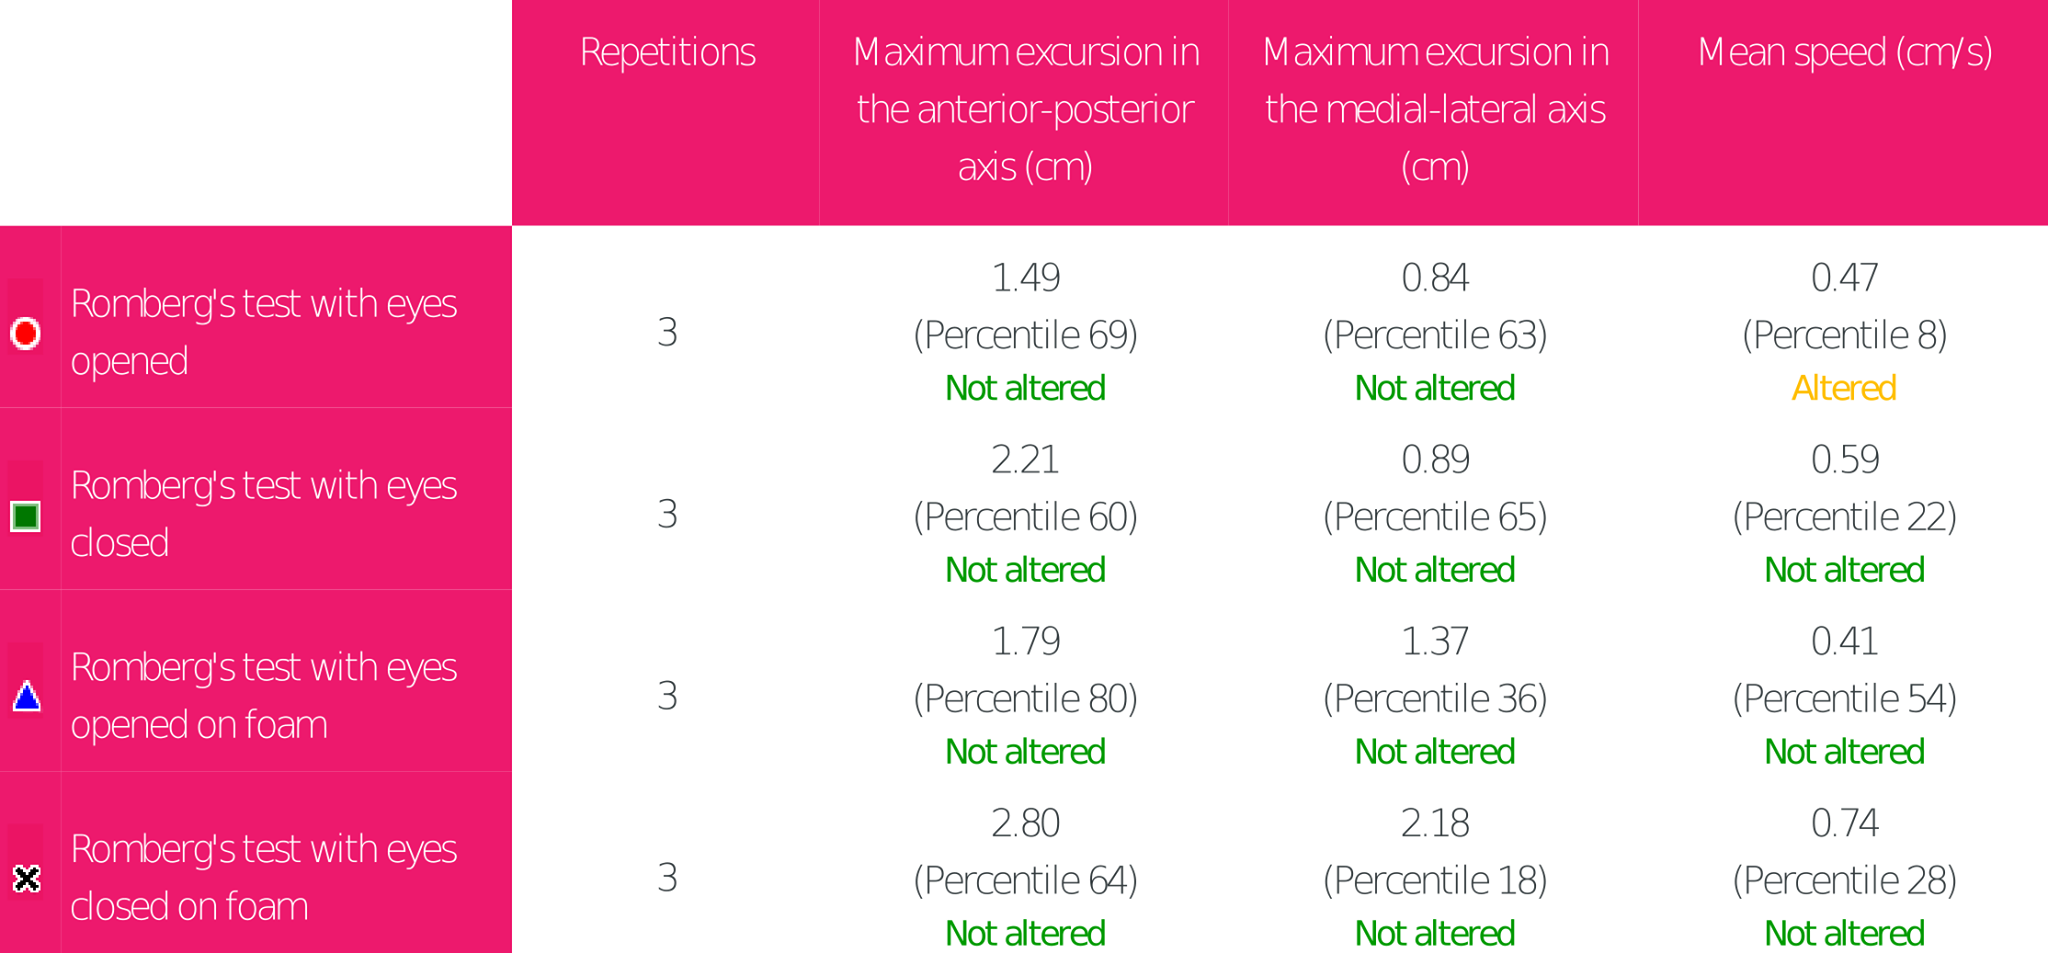
\includegraphics[width=1.0\textwidth]{figs/PTeste.png}
\\\footnotesize Nota: Imagem Adaptada de um teste preliminar realizado pelos autores desse trabalho
\end{figure}



Três protocolos de exercícios estão presentes no sistema de posturografia baseado na WBB: o Teste Clínico de Interação Sensorial modificado (mCTSIB), o teste de Limites de Estabilidade (LOS) e o Teste de Deslocamento de Peso Rítmico. O mCTSIB é uma versão simplificada do Teste de Organização Sensorial (\citeauthor{ford1995test}, \citeyear{ford1995test}) que pode ser implementado com placas de força fixas como no WBB. O mCTSIB requer que os participantes permaneçam imóveis por 30 segundos em quatro condições sensoriais diferentes: olhos abertos em uma superfície plana, olhos fechados em uma superfície plana, olhos abertos sobre uma espuma e olhos fechado sobre uma espuma. No Posturography Test, três repetições de cada condição são feitas para estimar a velocidade média e a média da excursão máxima nos eixos médio-lateral (ML) e ântero-posterior (AP).

O teste LOS estima a distância máxima que o paciente pode deslocar seu COP em oito direções (0$^{\circ}$, 45$^{\circ}$, 90$^{\circ}$, 135$^{\circ}$, 180$^{\circ}$, 225$^{\circ}$, 270$^{\circ}$ e 315$^{\circ}$). O teste RWS requer que os sujeitos desloquem ritmicamente seu COP nos planos ML e AP em três velocidades diferentes, enquanto atingem 80\% de seu limite de estabilidade em cada direção. O LOS deve ser realizado antes deste exercício para identificar esses limites (\citeauthor{llorens2015low}, \citeyear{llorens2015low}).

A fim de confirmar a ferramenta como substituta confiável para os sistemas de posturografia comerciais, Llorens et al. (\citeauthor{llorens2016posturography}, \citeyear{llorens2016posturography}) realizou um estudo para determinar a validade concorrente do sistema baseado no uso da WBB com outros testes clínicos de posturografia. A credibilidade da ferramenta foi quantificada através da confiabilidade inter e intra-avaliador, o erro padrão de medição e sua alteração mínima detectável. Um total de 144 indivíduos saudáveis (62 homens e 82 mulheres) com idade de 43,3  ±  18,6 anos
participaram do teste.  Os indivíduos foram classificados em sete grupos de acordo com suas idades por década de 10 a 80 anos e o desempenho médio de cada grupo em todos os testes foi calculado. Além disso, os indivíduos foram avaliados com o sistema de posturografia NedSVE/IBV e com vários testes de equilíbrio para determinar a validade concorrente da ferramenta com a avaliação experimental. Pacientes com acidente vascular cerebral também foram avaliados com o sistema baseado em WBB e seu desempenho foi comparado com o do grupo correspondente à idade, afim de avaliar o uso do sistema como ferramenta clinica. Ao fim do estudo o sistema mostrou uma validade concorrente moderada a alta com o outro sistema de posturografia. Quando comparado com os testes clínicos, a confiabilidade do sistema foi excelente em quase todas as medidas. Além disso, o sistema caracterizou com sucesso indivíduos com AVC quando comparados com à população saudável, atestando a viabilidade do seu uso como uma ferramenta clínica.




